\section{Conclusiones}

\fbox{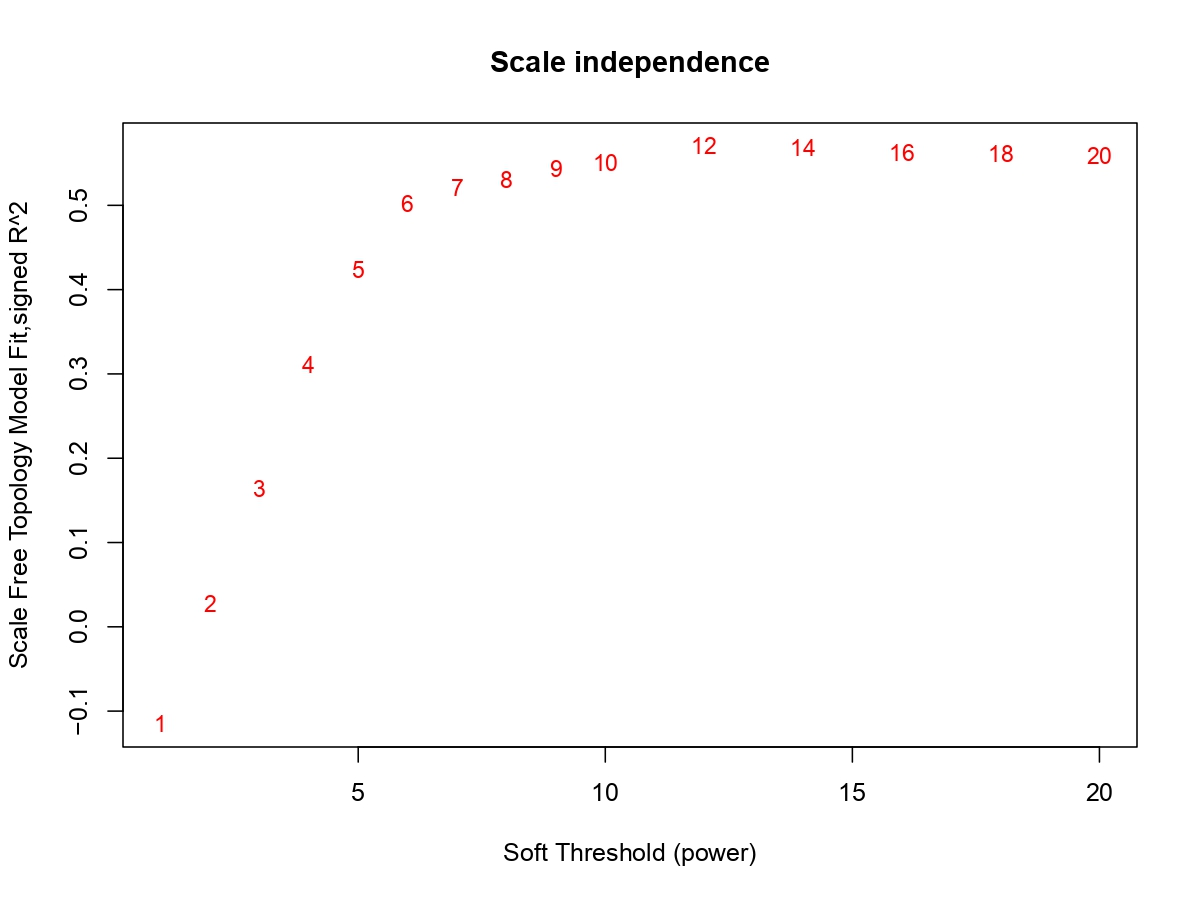
\includegraphics[width=0.9\textwidth]{figures/independenceScale_meanConnectivity1.jpg}}

\caption{independenceScale_meanConnectivity1}
\label{fig:sample_clustering}

\fbox{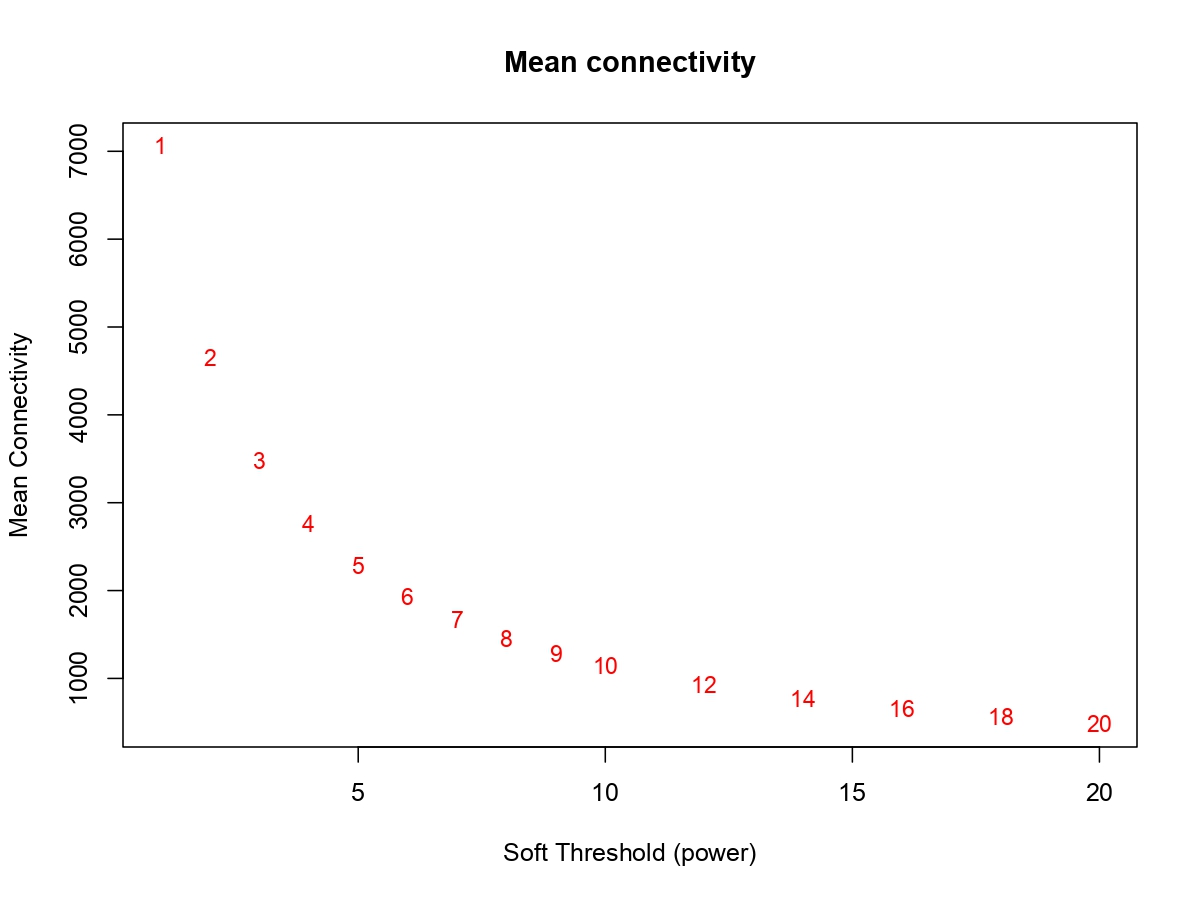
\includegraphics[width=0.9\textwidth]{figures/independenceScale_meanConnectivity2.jpg}}

\caption{independenceScale_meanConnectivity2}
\label{fig:sample_clustering}

Para el análisis de la topología de la red, lo primero que hemos hecho a nivel de implementación es la selección de umbrales. Posteriormente, transformamos el tipo de valores para todas las columnas, preocupándonos de que una función no detecta los valores si no son tipo \textit{NUMERIC}. Tras construir la red de genes y la identificaicón de los módulos, guardamos la información de la construcción de red.

\fbox{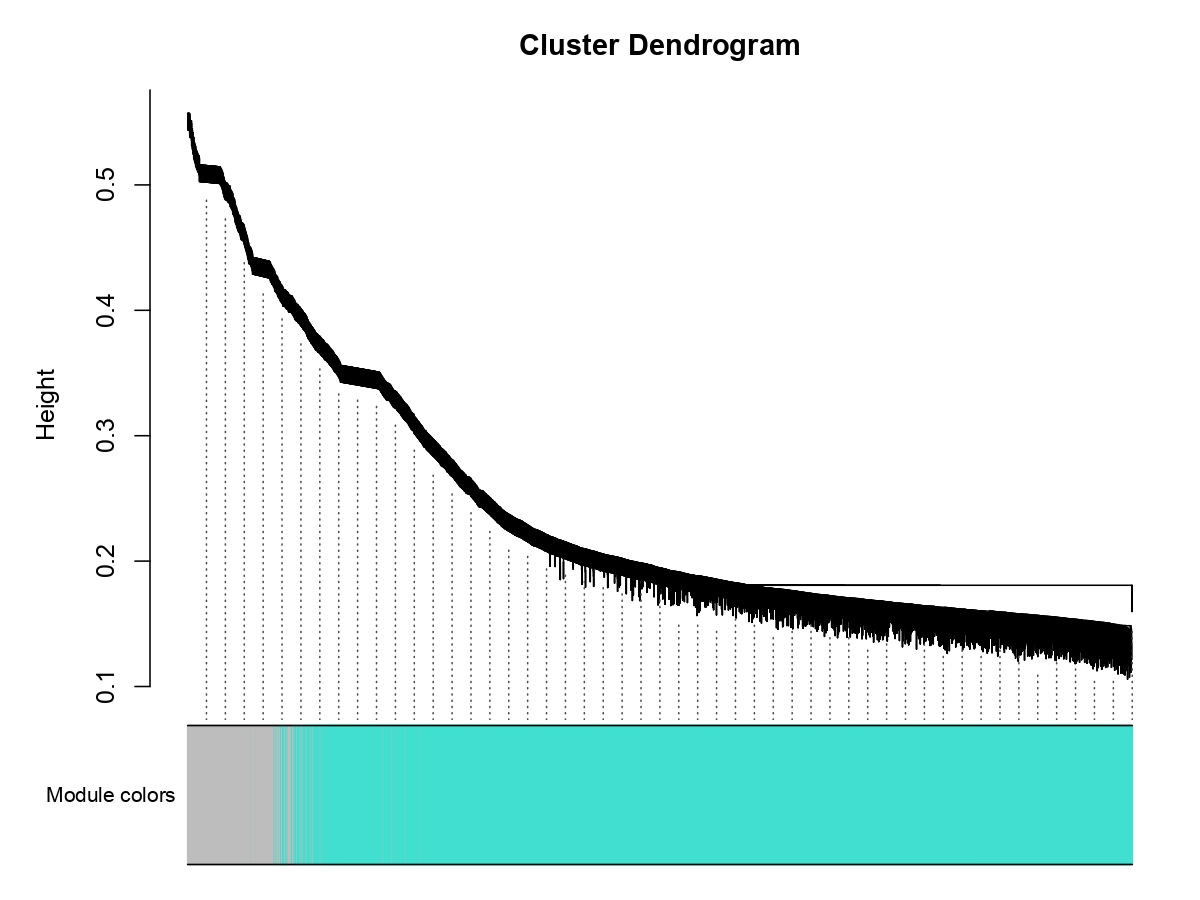
\includegraphics[width=0.9\textwidth]{figures/clusterDendrogram.jpg}}

\caption{Cluster Dendrogram}
\label{fig:sample_clustering}
